%!TEX encoding = UTF-8 Unicode
%!TEX root = ./../main.tex
%!TEX TS-program = xelatex

\chapter{Observation Pack} % Main chapter title
\label{cap:quattro}
Esistono molte varianti dell'algoritmo L* originariamente presentato da Angluin. L'algoritmo \ac{ObP} presentato da Falk Howar in \cite{Howar12} --presentato per le Mealy Machines ma comunque applicabile ai DFA -- si basa su alcune di queste varianti. Tecnicamente l'\ac{ObP} combina l'idea di usare un \ac{DT} per i linguaggi regolari \cite{Kearns94} con una versione localizzata della tabella di osservazione \cite{Schapire93}. Inoltre viene utilizzata una tecnica più efficiente di gestione del controesempio rispetto ad L*. Quindi l'\ac{ObP}  è in stretta correlazione con L*, e molti dei concetti introdotti nel capitolo \ref{cap:tre} rimangono validi. Anche \ac{ObP}, come L* è un algoritmo di \textit{active learning} nell'ambito dell'\ac{IIR} che garantisce di emmettere in output il \ac{DFA} minimo ( o uno ad esso isomorfo ) accettante \ac{L}. Anche in questo caso detto n il numero degli stati del DFA target minimo ed m la lunghezza del più lungo controesempio ritornato dal \textit{teacher} durante l'inferenza, il numero di \ac{MQ} sarà limitato da una funzione polinomiale di n ed m e il numero di \ac{EQ} linearmente da n. Nonostante L* sia il più noto algoritmo di \textit{active learning} l'\ac{ObP} ottiene prestazioni migliori dato che permette di diminuire il numero delle \ac{MQ}. Nell' \ac{ObP} il teacher appartiene ancora alla classe dei \ac{MAT}, in grado di rispondere ad \ac{EQ} e \ac{MQ}.
\section{Fondamenta teoriche}
Si parla di \textit{active learning} perchè il \textit{learner} attivamente può interrogare il \textit{teacher} sull'appartenenza o meno di alcune stringhe ad \ac{L}, in contrapposizione al \textit{passive learning} in cui le stringhe sono date a priori come in \textit{EDSM} ad esempio. Il \textit{learner} da un certo punto di vista si trova ad affrontare un problema di \textit{classificazione} cioè deve assegnare alcune stringhe ad un determinato stato di \ac{H}. L'ipotesi \ac{H}  ottenuta induttivamente sarà consistente con l'etichettatura degli esempi sottoposti al \textit{teacher}  fino al momento della creazione di \ac{H} ma produrrà una generalizzazione dato che in \ac{H} è possibile effettuare il \textit{parsing} di stringhe mai sottoposte al \textit{teacher}. Detto T il \ac{DFA} target,la \textit{classificazione} delle stringhe e la costruzione dell'ipotesi si basa sui risultati del teorema Myhill-Nerode (teorema \ref{teo:m-n}) che consente di:
\begin{enumerate}
\item Trovare un insieme $Sp \subset \Sigma^{*}$ di \textbf{prefissi}, detti \textbf{short prefix o access sequence},   in cui ogni short prefix è una stringa reppresentativa per una classe di equivalenza sulla relazione d'equivalenza $\simeq_{\lambda^{T}}$
 \item Trovare un insieme $V \subset \Sigma^{*}$ di \textbf{suffissi} che è sufficiente a realizzare la relazione di Nerode su \textit{Sp}, cioè tale che $s \not\simeq_{\lambda^{T}} \!\!s'$ implica $\lambda^{T}(sv) \neq \lambda^{T}(s'v) \text{ per } s,s' \in Sp \text{ e qualche } v \in V$ 
\end{enumerate}
Il teorema di Myhill-Nerode asserisce che un linguaggio $L(T) = \ac{L}$ è regolare se e solo se $\simeq_{\lambda^{T}}$ identifica un numero finito di classi d'equivalenza. $\simeq_{\lambda^{T}}$ agisce su due stringhe x e y che sono in relazione se non esiste nessuna stringa z tale che xz e yz, esattamente una delle due appartiene ad \ac{L}: quindi nella classe d'equivalenza ci saranno stringhe non distinguibili da nessuna altra stringa e che quindi rappresentano un unico stato dell'automa T. L'\ac{ObP} trova dei prefissi in cui ogni singolo prefisso è una stringa. contenuta in una specifica classe d'equivalenza (e vi è un prefisso rappresentativo, detto short prefix, per ogni classe d'equivalenza). Essendo  $L(T)=\ac{L}$ un linguaggio regolare, il numero di classi d'equivalenza è finito e sarà certamente possibile trovare un insieme di short prefix Sp . L'esistenza dell'insieme di suffissi V in 2 è garantita dal fatto che se esistono almeno due classi di equivalenza deve esistere almeno un suffisso che distingue le due classi d'equivalenza (che altrimenti sarebbero un'unica classe d'equivalenza). Quindi $\abs{V}$ è limitato dall'indice di $\simeq_{\lambda^{T}}$ cioè dal numero di stati del \ac{DFA} target.
\section{Costruzione dell'ipotesi}
L'\ac{ObP} mantiene due strutture dati rappresentative dell'ipotesi: il \ac{DT} e un insieme di componenti.
\subsection{Tabella di osservazione localizzata}
A differenza di L* in cui vi è un'unica tabella d'osservazione rappresentativa dell'ipotesi, in \ac{ObP} vi è una tabella di osservazione di dimensioni ridotte per ogni stato trovato fino a quel momento denotata come \textbf{componente}:
\begin{definizione*}[Componente] \label{def:obstable}Un componente C è una quadrupla $\Braket{U,u_0,V,OT}$ dove:\\\\
$U \subset \Sigma^{*}$ è un insieme finito di prefissi\\
$u_0 \in U$ è l'unico short prefix del componente\\
$V \subset \Sigma^{*}$ è un insieme di suffissi  $v_1,\dots,v_k$\\
$OT : U \times V \to \{0,1,*\}$ è una funzione così definita:\\\\
\centerline{$
OT[u][v] = 
\begin{cases}
1
& \text{se $uv \in \ac{L}$} \\
0 & \text{se $uv \notin \ac{L}$}\\
* & \text{altrimenti}
\end{cases}
$}   \\\\
Sia $u \in U$ e sia $\abs{V} = n$, si indica con row(u) la riga in OT indicizzata da u cioè $row(u)=OT[u][v_1] \cdot OT[u][v_2] \cdot \dots OT[u][v_n]$. Il componente è individuato dall'access sequence e quindi spesso lo si indica con $C_{u_{0}}$   
\end{definizione*}
Un componente approssima\footnote{Si parla di approssimazione perchè può accadere che alcuni prefissi che attualmente fanno parte dello stesso componente in futuro facciano parte di componenti diverse. Ciò è dovuto all'aggiunta di nuovi suffissi non ancora esaminati fino a quel momento. In ultima analisi ciò è dovuto al fatto che OT ha un dominio ristretto ad $U\times{}V$ anzichè $\Sigma^{*}$} la relazione di Nerode. Ogni componente rappresenta una classe di equivalenza: tutti i prefissi del componente fanno parte della stessa classe di equivalenza cioè   sono equivalenti (secondo OT) in base ai suffissi di quel componente. I valori di output di OT sono ricavati tramite delle \ac{MQ}. L'access sequence non è altro che un prefisso, possibilmente il più breve ma non necessariamente, rappresentativo del componente. Nell'ipotesi \ac{H} ad ogni componente  corrisponde uno stato. I prefissi di un componente sono tutte quelle stringhe che terminano nello stato dell'ipotesi rappresentato da quel componente. L'insieme di tutti i componenti è indicato con $C_I$, invece con Sp($C_I$) o semplicemente Sp si indica l'insieme delle access sequences di tutte le componenti. \textbf{Sp è prefix-closed}.
\subsubsection{Completezza}
La completezza garantisce che non ci siano comportamenti parzialmente (o totalmente) sconosciuti per prefissi presenti all'interno di una componente.
\begin{definizione*}[Componente completo] Un componente è completo se non ha \textit{buchi}. Un \textit{buco} in un componente è una coppia (u,v) tale che $OT[u][v] = *$.
\end{definizione*}
$C_I$ è completo se tutti i componenti sono completi.
L'eventuale incompletezza può essere eliminata mediante \ac{MQ} al \textit{teacher}.
\subsubsection{Chiusura}
La proprietà di chiusura di $C_I$ garantisce che tutti i prefissi di un componente sono equivalenti secondo la relazione di Nerode approssimata.

\begin{definizione*}[Componente chiuso] Un componente $\Braket{U,u_0,V,OT}$ è chiuso se $\text{row}(u) = \text{row}(u_0) \text{ per } \forall u \in U$.
\end{definizione*}
$C_I$ è chiuso se tutti i componenti sono chiusi.\\

La proprietà di chiusura su $C_I$ consente l'applicazione del teorema di Myhill-Nerode sulla relazione $\simeq_{OT}$ . La relazione di Nerode è soltanto approssimata in quanto la funzione OT non è definita su $\Sigma^{*}$ ma su un dominio più ristretto. Tuttavia, se le proprietà di chiusura  e completezza  su $C_I$ sono mantenute il teorema Myhill-Nerode è ancora valido e come visto in \ref{teo:m-n} assicura la costruzione di un \ac{DFA} la cui \textit{funzione di output} è quella su cui si basa la relazione di Nerode utilizzata che nella fattispecie è OT. Un ipotesi \ac{H} consistente con OT può essere costruita come nell'algoritmo \ref{alg:obp-buildautomaton}. L'eventuale non chiusura di un componente può essere eliminata con uno \textit{split} , che consiste nel dividere un componente in due componenti oppure uno stato in due stati (un componente corrisponde ad uno stato).

\begin{algorithm}
\caption{OBP-BUILDAUTOMATON}\label{alg:obp-buildautomaton}
\begin{algorithmic}[1]
\Statex
\Input a closed and complete components set $C_I$
\Output DFA $\Braket{\Sigma,Q,q_\epsilon,F_A,F_R,\delta}$
\State $Q \gets \{q_u :  \forall  u \in \text{Sp}(C_I)\}$
\State $q_\epsilon \gets \text{Component with short prefix } \epsilon $ \LineComment{Stato iniziale corrispondente al componente con short prefix $\epsilon$} 
\State $F_{\mathbb{A}} \gets \{q_u \in Q : \text{OT}[u][\epsilon] = 1\}$
\State $F_{\mathbb{R}} \gets \{q_u \in Q : \text{OT}[u][\epsilon] = 0\}$
\For{$q_u \in Q$}
     \For{$a \in \Sigma$} $\delta(q_u,a) \gets q_w \in Q : \text{row}(ua) = \text{row}(w)$
\LineComment{Da $q_u$ per a si va nello stato $q_w$ se ua è nel componente con short prefix w}     
     \EndFor
\EndFor
\State \textbf{end for}
\State \Return{$\Braket{\Sigma,Q,q_\epsilon,F_A,F_R,\delta}$}
\end{algorithmic}
\end{algorithm}

\subsection{Discrimination tree}
\begin{definizione*}[Discrimination tree]
Un \textit{discrimination tree} è un albero binario con radice definito come \ac{DT} = $\Braket{N,n_0,E,\tau,L}$ dove:\\\\
N è un insieme finito di nodi\\
$n_0 \in N$ è la radice dell'albero\\
$E \subseteq N \times N \times \mathbb{B}$ è l'insieme finito di archi\footnote{Si specifica per ogni arco se il secondo nodo è figlio destro o sinistro del primo nodo (rispettivamente 1 e 0)}\\
$\tau : N \to \Sigma^{*}$ assegna le etichette ai nodi\\
$L \subseteq N$ è l'insieme di foglie 
\end{definizione*}

\begin{figure}[htp]
	\centering
	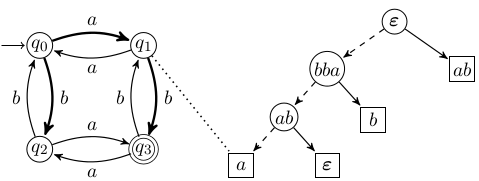
\includegraphics[ width=0.7\textwidth]{DTipotesi}
	\caption[Correlazione tra ipotesi e discrimination tree]{DFA ipotesi e possibile Discrimination Tree corrispondente}
   \label{fig:hdt}
\end{figure}
Un \ac{DT} è in stretta connessione con l'ipotesi come mostrato in figura \ref{fig:hdt}. C'è una corrispondenza biunivoca tra foglie nel \ac{DT} e stati in \ac{H}. Come si può vedere in figura  \ref{fig:hdt} alcune delle transizioni in \ac{H} sono disegnate in \textit{bold} perchè corrispondono ai prefissi che fungono da short prefix: nella fattispecie si ha $Sp=\{\epsilon,a,ab,b\}$. Le foglie sono etichettate con gli short prefix contenuti in Sp. I nodi interni invece sono etichettati con i suffissi $\in V \text{ di } C_I$ che consentono di \textit{discriminare} le foglie cioè stati diversi del \ac{DFA}. Il \ac{DT} assicura l'esistenza di un discriminatore per ogni coppia di foglie ( e quindi di short prefix e di stati) diverse, il \ac{LCA}. L' \ac{LCA} di due foglie a e b è incontrato nei rispettivi percorsi dai nodi verso la radice e rappresenta ,nei percorsi dalla radice verso a e b, il nodo in cui questi percorsi divergono come evidenziato in figura \ref{fig:lca}.\\Un'operazione fondamentale è il \textit{sift} di una stringa $x \in \Sigma^{*}$ nel \ac{DT} che consente di \textit{affondare} x all'interno dell'albero. Sia q un nodo interno etichettato con v ed A il \ac{DFA} target, il sifting di x  procede,partendo dalla radice, nel sottoalbero sinistro o nel sottoalbero destro di q a seconda del valore di $\lambda^{A}$(xv) (se è 0 si va nel sottoalbero sinistro). Questa procedura è ripetuta finchè una foglia è raggiunta. Ad esempio in figura \ref{fig:hdt} il \textit{sift} della stringa aba ---,che ha access sequence b, e che in \ac{H} termina nello stato $q_2$ --- tramite la valutazione nel \ac{DFA} target A di $\lambda^{A}(aba \cdot \epsilon)$ che da 0 (per questo si va a sinistra) e di $\lambda^{A}(aba \cdot bba)$ che produce 1 (per questo si va a destra)  arriva alla foglia con etichetta b (non casualmente, infatti b e aba sono transizioni che  nell'ipotesi giungono nello stesso stato e quindi sono nella stessa classe di equivalenza).Il \textit{sift} è descritto in dettaglio nell'algoritmo \ref{alg:sift} e nella sottosezione \ref{sub:fun}.
\subsection{Observation Pack}
\begin{definizione*}[Observation Pack]
Un Observation Pack è una tupla $\Braket{C_{I} , \ac{DT}}$
\end{definizione*}
Da cui deriva il nome dell'algoritmo. Un Observation Pack è chiuso e completo se $C_I$ è chiuso e completo.

\begin{figure}[htp]
	\centering
	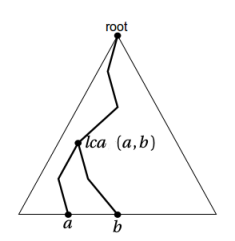
\includegraphics[ width=0.5\textwidth]{LCA}
	\caption[LCA di due nodi]{LCA di due nodi in un discrimination tree}
   \label{fig:lca}
\end{figure}
\section[Gestione Controesempio]{Gestione del controesempio}

\subsection{Classificazione}
\label{sub:cla}
Un controesempio è una stringa  w $\in \mathcal{L} \oplus L(\ac{H})$ che viene ritornato dal \textit{teacher} quando \ac{H} e il target differiscono. w va sfruttato dal \textit{learner} in qualche modo per produrre una nuova ipotesi \ac{H}. Esistono essenzialmente due modi per farlo: 
\begin{enumerate}
\item \textit{Metodi Suffix-based}. Aggiungono uno o più suffissi del controesempio all'insieme di suffissi dell'algoritmo provocando la non chiusura.
\item \textit{Metodi Prefix-based}. Aggiungono uno o più prefissi di un controesempio all'insieme di prefissi dell'algoritmo causando l'inconsistenza delle osservazioni, cioè una situazione di indeterminismo in \ac{H}.
\end{enumerate}
\ac{ObP} usa la prima strategia.Inoltre un'ulteriore classificazione sui metodi di gestione del controesempio viene effettuata in base a (1) se tutti o solo qualche suffisso (prefisso nel caso dei metodi \textit{prefix-based}) del controesempio sono impiegati e (2) questi suffissi (prefissi) sono applicati a tutti o solo a qualche prefisso (nell'accezione di prefisso rappresentante uno stato dell'ipotesi). Esistono diverse versioni di \ac{ObP} (e in generale anche per i metodi \textit{suffix-based}) in base  a quest'ulteriore classificazione:
\begin{itemize}
\item \textbf{AllGlobally}.\\Si aggiungono tutti i suffissi del controesempio all'insieme di suffissi V di ogni componente in $C_I$.
\item \textbf{OneGlobally}\\Si individua e si aggiunge un singolo suffisso del controesempio e lo si aggiunge all'insieme di suffissi V di ogni componente in $C_I$.
\item \textbf{OneLocally}\\Si individua e si aggiunge un singolo suffisso del controesempio ad un ben preciso componente.
\end{itemize}
In tutti e tre i casi l'aggiunta del suffisso (o dei suffissi) porterà alla non chiusura di almeno un componente e al conseguente \textit{split} che produrrà un nuovo stato nell'ipotesi.  In AllGlobally e OneGlobally è possibile far diventare l'insieme V globale dato che è uguale per ogni componente. Nella strategia OneLocally l'insieme V di suffissi differirà da componente a componente. Su come sia possibile individuare un singolo suffisso dal controesempio e l'esatto componente a cui bisogna aggiungere questo suffisso si rimanda al teorema \ref{teo:dec}.
Una classificazione simile è possibile per i metodi \textit{prefix-based}.
 La politica di gestione del controesempio è una differenza rilevante tra L* e \ac{ObP}. L* gestisce il controesempio in maniera poco sofisticata: usa un metodo \textit{prefix-based} in cui tutti i prefissi del controesempio sono aggiunti alla tabella di osservazione:quindi è una strategia AllGlobally dato che tutti i prefissi del controesempio sono usati in combinazione con un insieme di suffissi globale. Questa strategia causa l'inconsistenza di alcuni prefissi e per risolverla si aggiunge un suffisso che a sua volta causa una non chiusura e una promozione (un prefisso BLUE diventa RED). Lo svantaggio principale di questa strategia è che vengono aggiunti dei prefissi improduttivi che fanno aumentare il numero di \ac{MQ}. Invece con una strategia che aggiunge un solo suffisso (o un solo prefisso) è necessario fare delle \ac{MQ} per trovare il suffisso in questione dal controesempio ma il numero complessivo di \ac{MQ} risulterà sempre minore complessivamente ad una strategia AllGlobally come quella usata da L* (qui si fa riferimento alla versione originale di L* in \cite{Angluin87}. Esiste la variante OneLocally di L* in \cite{Kearns94} che determina un unico prefisso del controesempio  che genera inconsistenza, che viene risolta con l'aggiunta di un suffisso che causa uno \textit{split} nella loro versione del discrimination tree). 

\subsection[Decomposizione controesempio]{Decomposizione del controesempio}
Il seguente risultato fondamentale \cite{Schapire93} garantisce che dato qualsiasi controesempio esiste sempre un suffisso che discrimina due prefissi nello stesso componente e ne causa di conseguenza lo \textit{split}:
\begin{teorema}[Decomposizione del controesempio]\label{teo:dec} Sia H un'ipotesi, A il target, e $w \in \Sigma^{+}$ un controesempio ,cioè $\lambda^{A}(w) \neq \lambda^{H}(w)$. Allora esiste una decomposizione $\Braket{u,a,v} \in \Sigma^{*} \times \Sigma \times \Sigma^{*}$ tale che $w = u\!\cdot\! a\!\cdot\! v$ \text{ e } $\lambda^{A}(\lfloor u \rfloor_{H} a \cdot v) \neq \lambda^{A}(\lfloor ua \rfloor_{H} \cdot v)$ .
\end{teorema}  
Innanzitutto bisogna precisare che il controesempio non può essere mai $\epsilon$ perchè $\lambda^A(\epsilon) = \lambda^H(\epsilon)$ che segue da $\epsilon \in Sp$ e dall'invariante (I2) (vedasi sottosezione \ref{sub:corret}) e ciò giustifica l'assunzione $w \in \Sigma^{+}$ che si fa nel teorema \ref{teo:dec}. Si osservi che u e $\lfloor u \rfloor_{H}$ sono stringhe che terminano nello stesso stato di \ac{H}, lo stesso dicasi allora per ua e $\lfloor u \rfloor_{H}\cdot a$. Inoltre ua e $\lfloor ua \rfloor_{H}$ terminano nello stesso stato di \ac{H} da cui segue transitivamente che pure $\lfloor u \rfloor_{H}\cdot a$ e $\lfloor ua \rfloor_{H}$  terminano nello stesso stato dell'ipotesi \ac{H} ( e quindi appartengono anche allo stesso componente dato che c'è corrispondenza biunivoca tra stati dell'ipotesi e componenti). Quanto detto è schematizzato nella figura \ref{fig:con}. Ma il teorema \ref{teo:dec} afferma che $\lambda^{A}(\lfloor u \rfloor_{H} a \cdot v) \neq \lambda^{A}(\lfloor ua \rfloor_{H} \cdot v)$ il che significa che $\lfloor u \rfloor_{H}\cdot a$ e $\lfloor ua \rfloor_{H}$ --- che sono due stringhe che in \ac{H} terminano nello stesso stato --- nel target A terminano in due stati diversi. Quindi si è trovato il suffisso v che discrimina i due prefissi $\lfloor u \rfloor_{H} \cdot a$ e $\lfloor ua \rfloor_{H}$ e in più si sa che i due prefissi sono anche nello stesso componente.
\begin{figure}[htp]
	\centering
	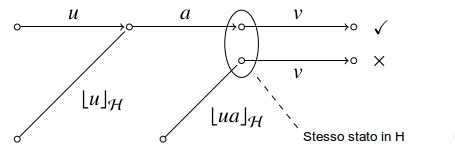
\includegraphics[ width=0.7\textwidth]{DiscriminazioneControesempio}
	\caption[Sfruttare il controesempio]{Sfruttare il controesempio}
   \label{fig:con}
\end{figure}
\subsubsection{Decomposizione del controesempio riformulata}
In \cite{StefCounterexample14} è descritto un framework che permette di riformulare il teorema \ref{teo:dec} in modo da facilitarne la comprensione della correttezza ed anche l'implementazione. Alcune funzioni si trovano nell'appendice \ref{app:due} e qui sono date per scontate.

Sia dato un controesempio $w \in \Sigma^{+}$ tale che $\abs{w}=m$. Dato che $\pi_{H}(w,m) \in Sp$ (si evince dalla definizione di w considerando che il controesempio è lungo m), dall'invariante (I2) (nella sottosezione \ref{sub:corret}) si ha $\lambda^{A}(\pi_{H}(w,m)) = \lambda^{H}(w)$ quindi $\alpha(m) = 1$ . Inoltre dato che $\pi_{H}(w,0) = w$ e $w$ è un controesempio si ha $\lambda^{A}(\pi_{H}(w,0)) \neq \lambda^{H}(w)$, quindi $\alpha(0) = 0$. Allora si può ricondurre il teorema \ref{teo:dec} nel trovare un undice i tale che $\alpha(i) \neq \alpha(i+1)$. Siccome $\alpha(0)=0 \text{ e } \alpha(1)=1$ sicuramente ci sarà un indice i in cui il valore di $\alpha$ passa da 0 ad 1 e ciò dimostra la correttezza e l'esistenza del suffisso. Il teorema \ref{teo:dec} può essere riformulato così:
\begin{teorema}[Decomposizione del controesempio riformulata] \label{teo:decr}Una politica di analisi del controesempio \textit{suffix-based} può essere riformulata come il problema di, data una funzione $\alpha: [0,m+1) \to \mathbb{B}$ con $\alpha(0)=0 \text{ e } \alpha(1)=1$, trovare un indice i, $0 \leq i < m$, soddisfacente $\alpha(i) \neq \alpha(i+1)$ 
\end{teorema}
Una volta trovato un indice i siffatto la decomposizione è u=$w_{[0,i)}$, a=$w_{i}$, v=$w_{[i+1,m)}$

\subsection[Metodi decomposizione controesempio]{Metodi di decomposizione del controesempio} Esistono diverse strategie per la ricerca del suffisso (o per i metodi \textit{prefix-based}) all'interno del controesempio. I parametri da tenere in considerazione nella valutazione di tali strategie sono il numero di \ac{MQ} effettuate e la dimensione del suffisso trovato. Infatti per valutare $\alpha(i)$ è necessaria una \ac{MQ} quindi l'impiego di un'euristica o di una politica che porta velocemente alla scoperta dell'indice i e quindi del suffisso permette di risparmiare il numero di \ac{MQ} da effettuare al \textit{teacher}. La dimensione dei suffissi\footnote{All'interno di un controesempio possono esistere più suffissi discriminatori, cioè molteplici indici i che permettono una decomposizione} è anch esso un parametro molto importante in quanto il suffisso trovato verrà aggiunto all'insieme dei suffissi dei componenti o del componente rispettivamente in OneGlobally e OneLocally, e anche al \ac{DT} (vedasi algoritmo \ref{alg:split}). Quando si navigherà il \ac{DT} , per esempio durante un sift, verranno fatte delle \ac{MQ} in cui parte della stringa è composta dall'etichetta di un nodo interno costituita da un suffisso; quindi il costo della \ac{MQ} crescerà linearmente con la dimensione del suffisso.

La strategia più semplice è quella che effettua una ricerca lineare in ordine discendente cioè partendo da $i = m-1$ che termina quando un valore i tale che $\alpha(i)=0$ è incontrato. Questo metodo assicura di trovare il suffisso più breve ma nel caso peggiore richiede m-1 \ac{MQ}. Anche se un costo lineare alla dimensione del controesempio sembra accettabile negli scenari reali non sempre lo è. In un contesto reale spesso capita di non avere la possibilità di effettuare un \ac{EQ} che va approssimata con un certo numero di \ac{MQ} nell'ambito del \textit{PAC-learning}. In questo scenario il controesempio tornato è una stringa di lunghezza non ottimale che può avere una lunghezza significativa. Esistono dei metodi che permettono di diminuire il numero di \ac{MQ} anche se spesso bisogna rinunciare alla lunghezza minima del controesempio ed accontentarsi di una lunghezza ottima.

\noindent

\begin{minipage}{0.48\textwidth}
\captionsetup{format=ruled,labelfont=bf}
%\flushleft
 \captionof{algorithm}{Binary-Search}\label{alg:bin}
   
    \begin{algorithmic}[0]
    \small
\Statex
\Input A counterexample w with $\abs{w}=m$
\Output Index i : $\alpha(i) \neq \alpha(i+1)$
\State $low \gets 0$
\State $high \gets m$
\While{$high-low>1$}
\State $mid\gets \lfloor \frac {low+high}{2} \rfloor$
\If{$\alpha(mid)=0$}
\State $low \gets mid$
\Else
\State $high \gets mid$
\EndIf
\EndWhile
\State \textbf{\quad\:\:end if}
\State \textbf{end while}
\State \textbf{return} $low$


\end{algorithmic}

  \kern2pt\hrule height.8pt\relax
\end{minipage}%
\hfill
\begin{minipage}{0.50\textwidth}
%\flushright
%\vspace{0pt}
\captionsetup{format=ruled,labelfont=bf}
  \captionof{algorithm}{Exponential-Search}\label{alg:exp}
  
    
    \begin{algorithmic}[0]
    \small
\Statex
\Input A counterexample w with $\abs{w}=m$
\Output Index i : $\alpha(i) \neq \alpha(i+1)$
\State $low\! \gets \!0,\, high\! \gets \!m,\, \text{\textit{ofs}}\! \gets \!1,\, found\! \gets \!\text{\textbf{false}}$
%\State $\text{\textit{ofs}} \gets 1, \:\: found \gets \text{\textbf{false}}$
\While{$high-ofs>0 \text{\textbf{ and }} \neg{}found$}
\If{$\alpha(high-ofs)=0$}
\State $low \gets high - ofs$
\State $found \gets \text{\textbf{true}}$
\Else
\State $high \gets high-ofs$
\State $ofs \gets 2 \cdot ofs$
\EndIf
\EndWhile
\State \textbf{\quad\:\:end if}
\State \textbf{end while}
\State \textbf{return} $\text{\textit{Binary-Search}}(\alpha,low,high)$

\end{algorithmic}
  
  \kern2pt\hrule height.8pt\relax
\end{minipage}





   
\subsubsection{Binary search}
Il metodo descritto nell'algoritmo \ref{alg:bin} è suggerito in \cite{Schapire93}. Esso impiega la ricerca binaria per trovare una decomposizione valida. Il numero di \ac{MQ} necessarie è $\lceil log_{2}(m) \rceil$ sempre, cioè non esiste un caso migliore ma il numero di \ac{MQ} è fisso perchè è necessario testare il valore di $\alpha()$ per due indici i contigui e ciò avviene solo alla fine della ricerca. La dimensione del suffisso trovata può anche essere molto più grande di quella minima.
\subsubsection{Exponential Search}
 Il metodo descritto qui e tutti quelli a seguire sono descritti in \cite{StefCounterexample14}.  La ricerca binaria ha lo svantaggio evidente che può essere tornato un  controesempio relativamente lungo: se il primo valore per \textit{mid} testato è tale che $\alpha(mid)=1$ il suffisso risultante sarà di lunghezza almeno   $\lceil m/2 \rceil$\footnote{La funzione $\alpha()$ non è necessariamente monotona quindi anche se $\alpha(mid)=1$ ci può essere un indice $i>m$ per il quale $\alpha(i)=0$ e quindi esserci un suffisso più breve}. Con \textit{exponential search}  si testano $\alpha(m-2^{0}),\alpha(m-2^{1}),\alpha(m-2^{2})$ eccetera, finchè non si trova un intervallo [l,h) per cui $\alpha(l)=0 \text{ e } \alpha(h)=1$ ed allora si chiamerà il metodo che usa la ricerca binaria descritto nell' algoritmo \ref{alg:bin} sui due indici l ed h. Nel caso peggiore(\textit{exponential search} non riesce a restringere l'intervallo cioè l resta 0 ed h resta m) questo metodo richiede $2\lfloor log_{2}(m) \rfloor$ \ac{MQ} , $\lfloor log_{2}(m)\rfloor$ per \textit{exponential search} e altrettante per la ricerca binaria.Nella maggior parte dei casi l'algoritmo termina molto prima e nel caso migliore ($\alpha(m-1)=0$) si effettua una singola \ac{MQ}. Per come funziona quest algoritmo favorisce il ritrovamento di suffissi più brevi rispetto alla ricerca binaria.\\
  \textit{Exponential Search} è presentato in dettaglio nell'algoritmo \ref{alg:exp}.
 
 \subsubsection{Partition Search}
\textit{Exponential search} può terminare velocemente e individuare suffissi molto brevi ma nel caso che  anche poche posizioni di $\alpha(m-2^{i}) = 1$ può essere svantaggiosa per via della rapida (anche per i piccolo),esponenziale, crescita dell'intervallo. Un approccio più bilanciato è quello di patizionare $\alpha$ in $\lceil log_{2}(m)\rceil$ intervalli, ognuno di lunghezza $s = \lfloor  \frac{m}{log_{2}m} \rfloor$. Poi i valori testati saranno $\alpha(m-s), \alpha(m-2s)$ eccetera, finchè un intervallo [l,h) soddisfacente $\alpha(l)=0 \text{ e } \alpha(h)=1$ è trovato. Quest intervallo sarà poi sottoposto al metodo di ricerca binaria per trovare un indice i in esso. In \textit{exponential search} a causa del passo esponenziale questo intervallo poteva risultare molto grande, in \textit{partition search} è di dimensione s. Quindi il numero di \ac{MQ} da effettuare nel caso peggiore con  \textit{partition search} è $log_{2}(s) = log_{2}(\lfloor  \frac{m}{log_{2}m} \rfloor)$ per via della ricerca binaria da eseguire sull'intervallo trovato più $\lfloor log_{2}(m)\rfloor$ (il numero di partizioni) \ac{MQ} per trovare l'intervallo. Quindi sono necessarie $\mathcal{O}(log_{2}(m))$ \ac{MQ}. \textit{Partition Search} è presentato in dettaglio nell'algoritmo \ref{alg:par}. Si osservi come il costo della ricerca binaria sia fisso (cioè è presente anche nel caso migliore) e dipendente da m. Quindi ci si aspetta che questo metodo funzioni meglio per controesempi non troppo grandi (m piccolo).

\subsubsection{Eager Search}
\textit{Eager Search} è una variante del metodo di ricerca binaria. Quest ultimo richiede sempre --- cioè non c'è un caso migliore o medio ma il numero di \ac{MQ} è sempre lo stesso --- $log_{2}(m)$ \ac{MQ}. Come accennato in precedenza il motivo è che il solo valore $\alpha(i)$ da solo non è sufficiente ma è necessaro testare anche $\alpha(i+1)$\footnote{perchè dal teorema \ref{teo:decr} si deve trovare un indice i per cui $\alpha(i) \neq \alpha(i+1)$}. La soluzione proposta in \textit{Eager Search} è di testare ogni volta il valore di $\alpha$ sia per i che per i+1 e vagliare se differiscono o detto in maniera più succinta che il
valore di $\beta$(vedasi \ref{equ:beta}) sia uguale ad 1. Nel caso peggiore siccome ogni valutazione di $\beta$ richiede 2 \ac{MQ} e il numero di valutazioni da fare è lo stesso della ricerca binaria (nel caso peggiore) sono necessarie $2log_{2}(m)$ \ac{MQ}. Tuttavia nel caso migliore solo 2 \ac{MQ} sono sufficienti e la ricerca può terminare molto prima di quella binaria. Questa strategia è affetta dallo stesso problema della ricerca binaria per quanto riguarda la dimensione dei suffissi tuttavia è possibile utilizzare \textit{Eager Search} in luogo della ricerca binaria sia in \textit{exponential search} che in \textit{partition search}. 

\noindent

\begin{minipage}{0.48\textwidth}
\captionsetup{format=ruled,labelfont=bf}
%\flushleft
 \captionof{algorithm}{Partition-Search}\label{alg:par}
   
    \begin{algorithmic}[0]
    \small
\Statex
\Input A counterexample w with $\abs{w}=m$
\Output Index i : $\alpha(i) \neq \alpha(i+1)$
\State $step \gets \lfloor \frac{m}{log_{2}(m)} \rfloor low \gets 0,\, high \gets m$
\State $found \gets \text{\textbf{false}}$
\While{$high\!-\!step\!>\!low \text{\textbf{ and }} \neg{}found$}
\If{$\alpha(high-step)=0$}
\State $low \gets high-step$
\State $found \gets \text{\textbf{true}}$
\State \text{\textbf{break}}
\Else
\State $high \gets high-step$
\EndIf
\EndWhile
\State \textbf{\quad\:\:end if}
\State \textbf{end while}
\State \textbf{return} $\text{\textit{Binary-Search}}(\alpha,low,high)$


\end{algorithmic}

  \kern2pt\hrule height.8pt\relax
\end{minipage}%
\hfill
\begin{minipage}{0.50\textwidth}
%\flushright
%\vspace{0pt}
\captionsetup{format=ruled,labelfont=bf}
  \captionof{algorithm}{Eager-Search}\label{alg:eag}
  
    
    \begin{algorithmic}[0]
     \small
\Statex
\Input A counterexample w with $\abs{w}=m$
\Output Index i : $\beta(i)=1$
\State $low \gets 0,\: high \gets m-1$
\While{$high > low$}
\State $mid\gets \lfloor \frac {low+high}{2} \rfloor$
\If{$\beta(mid)=1$}
\State \textbf{return} $mid$
\ElsIf{$\beta(mid)=0$}
\State $low \gets mid+1$
\Else
\State $high \gets mid-1$
\EndIf
\EndWhile
\State \textbf{\quad\:\:end if}
\State \textbf{end while}
\State \textbf{return} $low$
\end{algorithmic}
  
  \kern2pt\hrule height.8pt\relax
\end{minipage}
\section{L'algoritmo}
\label{sec:alobp}
\subsection{Funzionamento}
\label{sub:fun}
\ac{ObP} nella fase d'inizializzazione crea il componente corrispondente allo stato iniziale $C_{\epsilon} = \Braket{\Sigma \cup \{\epsilon\},\epsilon,\epsilon,\emptyset}$ ed il \ac{DT} è costituito solo dalla radice quindi $DT = \Braket{\{n_{\epsilon}\},n_{\epsilon},\emptyset,\tau(n_{\epsilon})=\epsilon,\{n_{\epsilon}\}}$ come si può vedere nell'algoritmo \ref{alg:obpp}. Dopodichè si chiama la funzione closePack() (vedasi algoritmo \ref{alg:clp}) che ha lo scopo di rendere chiusi e completi $C_{I}$ e modificare il \ac{DT} in modo da rappresentare la stessa ipotesi rappresentata da $C_{I}$. Si completano i $C_{I}$ e poi si ricerca un componente $C_{u}$ (questo in generale e non solo nella fase di inizializzazione dove l'unico componente è $C_{\epsilon}$) e un prefisso $u' \in C_{u}$ per cui $\text{row}(u) \neq \text{row}(u')$. Si seleziona il suffisso v per cui $OT[u][v] \neq OT[u'][v]$ e si divide $C_u$ chiamando la funzione \textit{split} (algoritmo \ref{alg:split}) che genererà un nuovo componente $C_{u'}$ e lo ritornerà a closePack(). In split() alcuni dei prefissi $U \in C_{u}$,che indichiamo con $x \in U$, ed esattamente quelli per cui $OT[x][v] \neq OT[u][v]$ vengono fatti migrare in $C_{u'}$ che nel frattempo è stato creato(cioè eliminati dal componente $C_{u}$ ed immessi in $C_{u'}$). Si procede poi a modificare di conseguenza anche il \ac{DT}: si individua il nodo foglia con etichetta u e lo si splitta nel senso che questo nodo foglia diventa un nodo interno con etichetta v (il suffisso, cioè il discriminatore) ed i suoi figli saranno due nodi foglia uno con etichetta u' e l'altro con etichetta u come si può apprezzare in figura\footnote{Per coerenza con il discorso fatto si consideri $v=v$, $b=u$,$b'=u'$} \ref{sub:split} (si stabilisce qual è il figlio sinistro e quale il destro in base al risultato della \ac{MQ} $\lambda^{A}(uv)$ nel target A, se questa fa zero u è il figlio sinistro del nuovo nodo con etichetta v altrimenti è il figlio destro). Si puntualizza che lo \textit{split} non necessita di \ac{MQ} aggiuntive e che l'insieme V del nuovo componente creato con lo \textit{splitting} è lo stesso dell'insieme V del componente da cui ha origine. A questo punto split() ritorna il componente in questione a closePack() che memorizza il componente trovato $C_{u'}$ in W\footnote{ (solo quando closePack() viene chiamato per la prima volta in assoluto ,immediatamente dopo la fase di inizializzazione, a W deve essere aggiunto anche $C_{\epsilon}$ (per esempio una coda)}. Finchè W non è vuoto si deve estrarre ed eliminare da W un componente , nella fattispecie $C_{u'}$, e concatenare l'access sequence del componente u' ad ogni simbolo di $\Sigma$ e per ogni stringa ottenuta effettuare il \textit{sift} (algortimo \ref{alg:sift}). Questo serve per assicurare in ogni caso la possibilità di costruire una nuova ipotesi \ac{H} in modo che per ogni nuovo componente aggiunto per ogni simbolo dell'alfabeto sia ben definito lo stato che viene raggiunto. Adesso si descrive in dettaglio come avviene il \text{sift} di una stringa x nel \ac{DT}: si parte dalla radice e si effettua la query nel target A $\lambda^{A}(\tau(n_{0})\cdot{}x)$ ,se da esito 0 si procede verso il sottoalbero sinistro altrimenti verso quello destro. Si continua in questa maniera finchè due situazioni possono presentarsi:
\begin{itemize}
\item Un nodo foglia $n_{x'}$ è incontrato. Significa che la stringa x in \ac{H} porta nello stato rappresentato dallo foglia in cui si è arrivati: detto $x'$ lo short prefix di questa foglia si ha che $x \in [x']_{\simeq_{OT}}$. Quindi si dovrà anche provvedere ad aggiungere x all'insieme U del componente $C_{x'}$. L'assegnazione della stringa come nuovo prefisso a un componente non è necessariamente definitiva perchè successivamente può accadere che la scoperta di un nuovo suffisso renda non chiuso un componente e per assicurare la chiusura si debba effettuare uno \text{split} che divide il componente in due parti e causando così possibilmente anche lo split di alcuni prefissi.
\item
Un nodo interno $n_{z}$ con un solo figlio e con etichetta $z$ è incontrato ma  $\lambda^{A}(xz)$ suggerisce di andare verso il percorso dove $n_{z}$ non ha figli. In questo caso deve avvenire la creazione di una nuova foglia $n_{x}$ con etichetta x come figlio del nodo $n_{z}$. Conseguentemente deve essere aggiunto $C_x$ a $C_I$. L'insieme di suffissi V di $C_x$ sarà inizializzato in OneLocally con i suffissi trovati lungo il percorso nel \ac{DT} per arrivare alla nuova foglia e con OneGlobally e AllGlobally  con i suffissi globali dell'algoritmo.\end{itemize}
Nel caso in cui  sift() torna un nuovo componente a closePack() quest ultimo va aggiunto in W. Si ripete il procedimento finchè W non è vuota. In ultima analisi l'algoritmo termina quando $C_{I}$ è completo (la non completezza è generata dal \textit{sifting} e anche l'eventuale non chiusura tranne alla prima iterazione dove è causata dal suffisso trovato nella decomposizione del controesempio). Si procede poi alla generazione dell'ipotesi \ac{H} come visto nell'algoritmo \ref{alg:obp-buildautomaton} e si effettua un \ac{EQ} cui il \textit{teacher} può rispondere dato che si assume che appartenga alla classe dei \ac{MAT}. Se il target A e l'ipotesi \ac{H} sono equivalenti l'algoritmo termina garantendo che \ac{H} sia il DFA minimo e l'equivalenza di A e \ac{H} altrimenti verrà tornato un controesempio che verrà sfruttato per trovare un suffisso discriminante due prefissi appartenenti allo stesso componente (e con uno dei prefissi ,diciamo x, $: x \in Sp$). Se si usa OneLocally si aggiunge il suffisso all'insieme V di $C_{x}$, con OneGlobally si aggiunge il suffisso all'insieme V che sarà globale per tutte le componenti. Con la strategia AllGlobally non è necessario effettuare la decomposizione del controesempio in quanto si aggiungeranno tutti i suffissi del controesempio all'insieme di suffissi V globale e comune a tutte le componenti ma è chiaramente una strategia controproducente. L'aggiunta del suffisso v garantisce la non chiusura ad ogni  `` generazione  '' e quindi l'aggiunta di almeno un nuovo componente, e quindi stato, mediante lo \textit{split}.

\begin{algorithm}
\caption{OBP-SIFT}\label{alg:sift}
\begin{algorithmic}[1]
\Statex
\Input a $DT=\Braket{N,n_0,E,\tau,L}$, $C_I$ , new prefix $u \in \Sigma^{*}$   
\Output A new component or  ``OK''
\State $n=n_0$
     \While{$n \notin L$}
     \State $v \gets \tau(n)$
     \State $o \gets MQ(uv)$ \Comment{$MQ(uv) = \lambda^{A}(uv)$}
     \If {$ \exists (n,n',o) \in E$} \Comment{Se n ha un figlio nella direzione indicata da o}
     \State $n \gets n'$
     \Else \Comment{Il nodo n non ha figli nella direzione indicata da o}
     \State Create new node $n_u$
     \State $N \gets N \cup \{n_u\},\quad E \gets E \cup \{(n,n_u,o)\}$
     \State $\tau(n_u)=u$
     \State $\text{Create component }  C_u$ \LineComment{Aggiungi a $C_u$ lo short prefix u e i suffissi secondo la strategia usata}
     \State \textbf{return} $C_u$
     \EndIf  
     \EndWhile
      \State \textbf{end while}
     \LineComment{Se si è qui significa che si è arrivati a una foglia}
     \State $u'=\tau(n)$ \Comment{Si prende lo short prefix del nodo n}
     \State $\text{add u to } C_{u'}$ 
     \LineComment{aggiungere il prefisso al componente solo se il prefisso non è già presente}
    \State \textbf{return} ``OK'
\end{algorithmic}
\end{algorithm}

Inoltre a differenza di L* in \ac{ObP} è possibile sfruttare più volte lo stesso controesempio. In L* tutti i prefissi del controesempio  compreso il controesempio stesso vengono aggiunti alla tabella di osservazione e la nuova ipotesi generata è consistente con essi e quindi alla successiva `` generazione  '' il controesempio precedente non è più riutilizzabile perchè difatti non è più in \ac{L} $\oplus$ L(\ac{H}). In \ac{ObP} invece viene aggiunto un solo suffisso del controesempio e quindi potrebbe accadere che alla successiva `` generazione  '' sia ancora un controesempio utilizzabile per trovare un altro suffisso che produca la non chiusura. Ciò può fare risparmiare molte \ac{EQ} al costo di una \ac{MQ} aggiuntiva per ogni `` generazione  '' (perchè è necessario testare se il controesempio è ancora tale).

\begin{algorithm}
\caption{OBP-SPLIT}\label{alg:split}
\begin{algorithmic}[1]
\Statex
\Input a $DT=\Braket{N,n_0,E,\tau,L}$, $C_I$ , a component $C_{u_{0}}=\Braket{U,u_0,V,OT}$, a prefix $u \in U$ , a suffix $v \in V : OT[u_0][v]) \neq OT[u][v]$
\Output A new component
\State $\text{Create component } C_u=\Braket{\emptyset,u,V,\emptyset}$
     \For{$u' \in U$}
     \If {$OT[u_0][v] \neq OT[u'][v]$}
     \State $\text{Transfer u' from } C_{u_{0}} \text{ to } C_{u} $ \Comment{Trasferire significa eliminare da $C_{u_{0}}$}
     \EndIf
     \EndFor
     \State \textbf{end for}
      \LineComment{Adesso a seguire le modifiche da apportare al discrimination tree}
      \State Let $n \in L$ where $\tau(n)=u_0$ \Comment{Seleziona la foglia con etichetta $u_0$}
      \State $\tau(n) = v$ \Comment{Modifica l'etichetta del nodo con quella del suffisso discriminante}
      \State Create new node $n_u$
      \State Create new node $n_{u_{0}}$
      \State $N \gets N \cup \{n_u,n_{u_{0}}\}$
      \State $\tau(n_u) = u$
      \State $\tau(n_{u_{0}}) = u_0$
      \State $E \gets E \cup \{(n,n_u,OT[u][v])\} \cup \{(n,n_{u_{0}},OT[u_0][v])\}$
    \State \textbf{return} $C_u$
\end{algorithmic}
\end{algorithm}



\begin{algorithm}
\caption{OBP-CLOSEPACK}\label{alg:clp}
\begin{algorithmic}[1]
\Statex
\Input a observation pack $\Braket{DT,C_{I}}$
\Output ipotesi H
\State $W \gets \emptyset $ \text{ (only in first call ever $W \gets \{C_{\epsilon}\}$)} 
     \While{$C_{I} \text{ is unclosed or incomplete }$} \label{lin:clpunclosed}
     \State Complete $C_I$
     \State Let $C_{u_{0}} = \Braket{U,u_0,V,OT} \text{ with } u \in U, v \in V : OT[u_0][v] \neq OT[u][v]$ \label{lin:clpsuffix}
     \State $C_u = $ \Call{OBP-SPLIT}{$DT,C_I,C_{u_{0}},u,v$}
     \State $W \gets W \cup \{C_u\}$
     \While{$W \neq \emptyset$}
     \State $C_u \gets poll(W)$ \LineComment{Estrai un componente secondo una qualche politica ad esempio FIFO}
     \For{$a \in \Sigma$}
     \State $C = $ \Call{OBP-SIFT}{$DT,C_I,ua$}
     \If{$C \neq$ ``OK''}
     \State $W \gets W \cup C$
     \EndIf
    
     \EndFor
      \State \textbf{end for}
     
     \EndWhile
     \State \textbf{end while}
    
    \EndWhile
    \State \textbf{end while} 
    
    \State $H= $ \Call{OBP-BUILDAUTOMATON}{$C_{I}$}
    \State \textbf{return } H
     
\end{algorithmic}
\end{algorithm}

\begin{algorithm}
\caption{OBSERVATION PACK}\label{alg:obpp}
\begin{algorithmic}[1]
\Statex
\Input alfabeto $\Sigma$ 
\Output minimal DFA H : L(H)=\ac{L}  
\State $C_{\epsilon}=\Braket{\Sigma \cup \{\epsilon\},\epsilon,\epsilon,\emptyset}$
\State $C_I = C_{\epsilon}$ 
    \State $DT = \Braket{\{n_{\epsilon}\},n_{\epsilon},\emptyset,\tau(n_{\epsilon})=\epsilon,\{n_{\epsilon}\}}$
    \Loop
    \State H = \Call{OBP-CLOSEPACK}{$DT,C_I$}
    \State w = \Call{EQ}{H}
    \If{ w = ``OK''}
    \State \textbf{return} H 
    \EndIf
    \State \textbf{end if}
     \If{AllGlobally}
    \State Add all suffixes of w to V of all components in $C_I$
    \State \textbf{continue}
    \EndIf
    \State \textbf{end if}
    \State Split w with a decomposition method in uav : $\lambda^{A}(\underbrace{\lfloor u \rfloor_{H}a}_{p} v) \neq \lambda^{A}(\underbrace{\lfloor ua
     \rfloor_{H}}_{u'}v)$
     \Statex \quad \: tale che $p \in C_{u'}$
    \If{OneGlobally}
    \State Add v to V of all components $\in C_I$ \label{lin:addsuffixes}
    \EndIf
    \State \textbf{end if}
    \If{OneLocally}
    \State Add v to V of $ C_{u'}$
    \EndIf
    \State \textbf{end if}
    \EndLoop
    \State \textbf{end loop}
     
\end{algorithmic}
\end{algorithm}

\subsection{Correttezza}
\label{sub:corret}
La correttezza dell' \ac{ObP} scaturisce dal mantenimento di tre \textit{\textbf{invarianti d'apprendimento}} :
\begin{enumerate}[label=\textbf{{(I}\arabic*{)}}]
  \item $u \neq u' \in Sp$ corrispondono a stati differenti nel \ac{DFA} target A cioè $A[u] \neq A[u']$.
  \item Ogni stato q in \ac{H} è accettante se e solo se ``parsando'' $\lfloor q \rfloor_{H}$ nel target A si termina pure in uno stato accettante. In simboli: $\forall q \in Q^{H} : q \in  F_{\mathbb{A}}^{H} \Leftrightarrow f_{Sp}(q) \in F_{\mathbb{A}}^{A}$
  \item Transizioni in \ac{H} puntano allo stato corretto nel target, se quest ultimo è già stato scoperto dal \textit{learner}: $\forall q \in Q^{H}, a \in \Sigma \text{ si ha } \delta^{A}(f_{Sp}(q),a) \in A[Sp] \implies f_{Sp}(\delta^{H}(q,a)) = \delta^{A}(f_{Sp}(q),a)$
\end{enumerate}
E' evidente che la scoperta di nuovi short prefix in Sp mantenendo la condizione (I1)  porterà alla scoperta di tutti gli stati nel target A (dato che sono finiti per il teorema di Myhill-Nerode descritto in \ref{teo:m-n}). Le condizioni (I2) ed (I3) garantiscono che $f_{Sp}$ è un isomorfismo .In L* vi è una violazione della condizione (I1) perchè può accadere che più di uno short prefix (più di uno stato RED) rappresentino lo stesso stato nel target. Il requisito di consistenza tuttavia garantisce che uno qualsiasi di questi può essere scelto come rappresentativo dello stato target.\\

Si dimostra che le tre \textit{invarianti} sono possedute dall'algoritmo \ac{ObP}:
\begin{enumerate}[label=\textbf{{(I}\arabic*{)}}]
\item Siano u e $u' \in Sp \text{ e } u \neq u' $,  allora essendo in due componenti diversi esiste un suffisso v che distingue u e $u'$ cioè tale che $\lambda^{A}(uv)=OT[u][v] \neq \lambda^{A}(u'v)=OT[u'][v]$. Quindi si ha anche $\lambda_{A[u]}^{A}(v) \neq \lambda_{A[u']}^{A}(v)$ e quindi $A[u] \neq A[u']$
\item  Sia $u=\lfloor q \rfloor_{H} $ l'access sequence di uno stato $q \in Q^H$.  Si ha allora che $q \in F_{\mathbb{A}}^{H} \iff$\!\!\footnote{Nel caso della strategia OneGlobally è lampante capire che in ogni componente ci sarà sempre il suffisso $\epsilon$ essendo questo già presente in fase d'inizializzazione. Utilizzando OneLocally accade lo stesso perchè i suffissi da aggiungere ad un nuovo stato (rappresentato da una access sequence e da un componente) sono quelli incontrati durante il \textit{sifting} dell'access sequence nel discrimination tree e quindi si passa sempre dalla radice che contiene il suffisso $\epsilon$} $OT[u][\epsilon]=1$.  Dato che $OT[u][\epsilon]=\lambda^{A}(u\cdot\epsilon)=\lambda_{A[u]}^{A}(\epsilon)$ si può concludere che $q \in  F_{\mathbb{A}}^{H} : u=\lfloor q \rfloor_{H} \Leftrightarrow A[u]$\footnote{è uguale a $f_{Sp}(q)$} $\in F_{\mathbb{A}}^{A}$
\item Sia dato uno stato $q \in Q^{H} $ tale che $u = \lfloor q \rfloor_{H}$, il successore di q per il simbolo $a \in\Sigma$ è determinato con il \textit{sifting} di ua nel \ac{DT}. Sia lo stato con access sequence $u'$ il risultato di questa operazione di \textit{sifting}, si definisce allora $\delta^{H}(q,a) = H[u']$. Se però nel target A questa transizione è errata cioè $\delta^{A}(A[u],a) \neq A[u']$, si sa per certo che il successore reale sul simbolo $a$ cioè  $A[ua]$ non è ancora stato scoperto, quindi (I3) è preservata: si noti che \textit{siftando} ua nell'albero, arrivando ad $u'$ si escludono definitivamente  gli altri  stati scoperti fino a quel punto $A[Sp\textbackslash \{u'\}]$ come possibili successori sul simbolo $a$ di $A[u]$. 
\end{enumerate}
Ciò dimostra la correttezza dell' \ac{ObP} ma tramite quanto detto sopra si dimostra solo che \ac{H} ed A sono isomorfi senza assumere la canonicità per \ac{H}. Infatti in generale  A non è un \ac{DFA} minimo e secondo quanto detto finora non si può dedurre che \ac{H} sia minimo ma solo isomorfo  ad A. Inoltre a causa del maccanismo di gestione del controesempio non vi è la garanzia che l'insieme di suffissi sia \textit{suffix-closed} dato che viene aggiunto solo un suffisso del controesempio. Quanto detto causa anche la generazione di ipotesi intermedie non minime. Tuttavia applicando l'euristica di utilizzare più volte lo stesso controesempio finchè da esso non è più possibile estrarre un suffisso discriminante è garantito che l'ipotesi finale è un \ac{DFA} canonico \cite[p. 25]{Stef11}. Esiste un'ottimizzazione che tramite  il concetto di \textit{semantic suffix closdness} ,sempre in \cite{Stef11} , assicura che anche le ipotesi intermedie prodotte siano canoniche ed il meccanismo che permette di scoprire dei nuovi suffissi da quelli esistenti in modo da ottenere la \textit{semantic suffix closdness} permette di risparmiare anche delle \ac{EQ} e \ac{MQ} perchè permette di scoprire nuovi suffissi discriminanti e nuovi stati senza costi aggiuntivi in termini di \ac{EQ} ed \ac{MQ} (vi è però il tempo di esecuzione aggiuntivo dell'algoritmo per garantire la \textit{semantic suffix closdness} ).


\subsection{Complessità computazionale}
Il tempo di esecuzione degli algoritmi di \textit{active learning} è quasi sempre un polinomio di grado piccolo dipendente dalla dimensione dell'alfabeto k, il numero di stati  del \ac{DFA} canonico  equivalente ad \ac{L} che qui si indica con $n$ , e la lunghezza del controesempio $m$ con cui si indica la lunghezza del più lungo controesempio tornato dal \textit{teacher}. Il tempo di esecuzione è quasi sempre dominato dal tempo speso nell'effettuare  \ac{MQ} ed \ac{EQ} \footnote{Talvolta si conta anche il numero di simboli contenuto in tutte le stringhe per cui si effettua una \ac{MQ} per pesare il costo di una \ac{MQ} dato che è lineare con la lunghezza} e quindi contare quest ultime può essere sufficiente per analizzare le prestazioni dell'algoritmo. In quest'ottica in \cite[p. 20]{Howar12} si trova un'analisi dell' \ac{ObP} nelle sue varie forme per le  Mealy machines confrontando i risultati con L*. Questi risultati vengono qui applicati ai \ac{DFA} e riportati nella tabella \ref{tab:mqa}. Dato che per tutti gli algoritmi il numero di \ac{EQ} è limitato da $\mathcal{O}(n)$ l'analisi delle \ac{EQ} viene omessa. Infine si noti come l'analisi venga effettuata nel caso peggiore.

Per tutti gli approcci il numero di suffissi necessari per distinguere tutti gli stati è limitato da $n$ dato che ogni aggiunta di un suffisso determina almeno uno \textit{split} e l'individuazione di almeno un nuovo stato (stati che sono al massimo n). Il numero di prefissi in tutte le componenti per \ac{ObP} è al più $n \cdot k$ perchè al più si hanno n componenti (n stati), se da ogni stato si hanno k transizioni il numero di transizioni totali sarà $n \cdot k$ (i prefissi di uno stato sono le transizioni che finiscono in quello stato). La dimensione della tabella di osservazione o meglio la somma delle dimensioni di tutte le tabelle di osservazione di ogni componente è allora $nk \cdot n$ (numero prefissi $\cdot$ numero suffissi). Per AllGlobally si aggiungono tutti gli $m$ suffissi di ogni controesempio, e lo si fa n volte quindi si avranno $n \cdot m$ suffissi con una tabella di dimensione $nk \cdot nm$. Per OneLocally e OneGlobally vi è da aggiungere il numero di query fatte durante la ricerca del suffisso che nel caso della ricerca binaria è $log_{2}(m)$ effettuate n volte. Per la dimensione della tabella di L* si faccia riferimento alla sottosezione \ref{subsub:comcom}.

\begin{table}[htp]
\centering
\[ 
\begin{array}{lcc} 
\toprule
\text{Algoritmo} & \text{Dimensione tabella} & \text{Membership queries}  \\
\midrule  
\text{L*}  &  (k + 1)\cdot(n + m(n − 1))\cdot n & \mathcal{O}(n^{2}km) \\
\text{AllGlobally}  &  nk\cdot nm & \mathcal{O}(n^{2}km) \\
\text{OneLocally}  &  nk\cdot n & \mathcal{O}(n^{2}k) \\
\text{OneGlobally}  &  nk\cdot n & \mathcal{O}(n^{2}k) \\

\bottomrule
\end{array}
\]
 \caption[Complessità membership queries ObP]{Complessità delle membership queries per le differenti varianti di ObP}
\label{tab:mqa}
\end{table}  

Tuttavia i risultati evidenziati nella tabella \ref{tab:mqa} ed anche quelli omessi per le \ac{EQ} costituiscono solo un limite superiore, il lavoro sperimentale in \cite[p. 22-23]{Howar12} mette meglio in evidenza le differenze tra i vari algoritmi. OneLocally è l'algoritmo con il minore numero di \ac{MQ} dato che il suffisso discriminante è aggiunto solo ad un componente e quindi sarà necessario completare solo la tebella di osservazione di questo componente ,e nonostante OneLocally e OneGlobally abbiano lo stesso ordine di grandezza per il numero di \ac{MQ} fatte al crescere dei parametri la differenza in termini di \ac{MQ} è notevole. In OneLocally tuttavia come detto in \cite[p. 23]{Howar12} il numero delle \ac{EQ} aumenta drasticamente rispetto a OneGlobally anche se in numero  pur sempre limitato dal numero di stati del \ac{DFA} minimo equivalente ad \ac{L}. L* effettua un numero di \ac{EQ} quasi sempre minore (seppur di poco) di OneGlobally ma un numero di \ac{MQ} sempre molto maggiore sia a OneLocally che a OneGlobally. AllGlobally consente di effettuare un numero di \ac{EQ} quasi sempre leggermente inferiore anche ad L* ma il numero di \ac{MQ} è sempre molto elevato anche rispetto ad L*.
\subsection{Discrimination tree vs Tabella di Osservazione localizzata}
 In figura \ref{sub:tol} vi è la rappresentazione della tabella di osservazione per
 \begin{figure}[htp]
\centering
\subfloat[\emph{Tab. Osservazione L*}][\label{sub:tol}]
{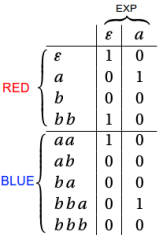
\includegraphics[width=.45\textwidth,height=6cm,keepaspectratio]{OBTLSTAR}} \quad
\subfloat[\emph{DFA ipotesi}.][\label{sub:dfah}]
{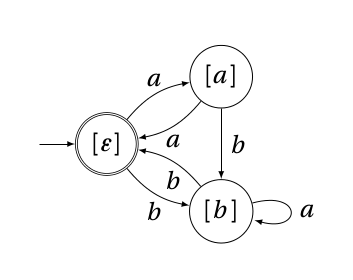
\includegraphics[width=.45\textwidth]{DFALstar}}
\caption{DFA ipotesi e corrispondente tabella di osservazione in L*}
\label{fig:dfal}
\end{figure} 
l'algoritmo L* per il \ac{DFA} in figura \ref{sub:dfah}. I prefissi RED distinti tra di loro $\{\epsilon,a,b\}$ (cioè con row() distinte tra di loro) sono gli short prefix delle classi di equivalenza che hanno una corrispondenza con gli stati del \ac{DFA}. I prefissi BLUE sono invece delle stringhe appartenenti ad una delle classi di equivalenza (un prefisso BLUE x termina nello stato rappresentato da uno stato RED r ed appartiene alla sua classe di equivalenza se row(r)=row(x) ). Il \ac{DT} è una rappresentazione della tabella di osservazione scevra da ridondanze come si può apprezzare in figura \ref{sub:dis}. Infatti a parte lo short prefix superfluo bb,  nella tabella di osservazione di L* non tutti i suffissi sono necessari per distinguere le varie classi di equivalenza (gli stati RED). Ad esempio il singolo suffisso  $\epsilon$ da solo è sufficiente per distinguere $[\epsilon]$ dalle altre classi di equivalenza. Lo scopo di un \ac{DT} è di eliminare queste ridondanze ed organizzare le osservazioni delle passate \ac{MQ} in una maniera efficiente in modo da consentire efficientemente il \textit{sifting} di una stringa.
 \begin{figure}[htp]
\centering
\subfloat[\emph{Discrimination Tree}][\label{sub:dis}]
{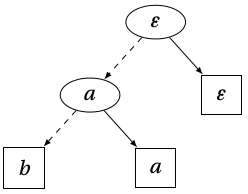
\includegraphics[width=.45\textwidth,height=6cm,keepaspectratio]{DTLSTAR}} \quad
\subfloat[\emph{Split}.][\label{sub:split}]
{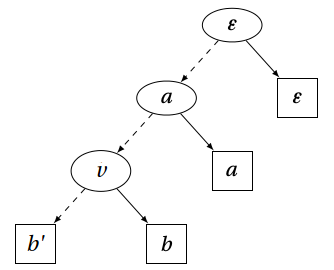
\includegraphics[width=.45\textwidth]{Split}}
\caption{Discrimination Tree e split di uno stato}
\label{fig:diss}
\end{figure} 
Nella tabella \ref{tab:com} vi è l'insieme di componenti di \ac{ObP} corrispondente alla tabella di osservazione per OneGlobally anche se è solo un esempio e molti dei prefissi presenti in L* potrebbero non essere presenti in \ac{ObP}. 
\begin{table}[htp]
\centering 
\begin{tabular}{|l|c|c|} 
\hline
$C_{\epsilon}$ & $\epsilon$ & $a$  \\
 \hline  
$\epsilon$  &  1 & 0 \\
\hline 
aa  &  1 & 0 \\
bb  &  1 & 0 \\
\hline
\end{tabular}
\quad
\begin{tabular}{|l|c|c|} 
\hline
$C_{a}$ & $\epsilon$ & $a$  \\
\hline
$a$ & 0 & 1  \\
 \hline  
$bba$  &  0 & 1 \\
\hline
\end{tabular}
\quad
\begin{tabular}{|l|c|c|} 
\hline
$C_{b}$ & $\epsilon$ & $a$  \\
\hline
$b$ & 0 & 0  \\
 \hline  
$ab$  &  0 & 0 \\
$ba$  &  0 & 0 \\
$bbb$  &  0 & 0 \\
\hline
 \end{tabular}
 \caption[Insieme di componenti]{Insieme di componenti}
\label{tab:com}
\end{table}  
 
Sia il \ac{DT} che $C_I$ sono rappresentativi dell'ipotesi e quindi vi deve essere in ogni momento coerenza anche tra \ac{DT} e $C_I$ oltre che con l'ipotesi. Infatti per ogni foglia nell'albero c'è un corrispondente componente  in $C_I$, l'etichetta della foglia corrisponde all'access sequence di quel componente. Entrambe le strutture dati sono rappresentative dell'ipotesi.
A questo punto ci si potrebbe chiedere perchè utilizzare sia un \ac{DT} che $C_I$ per rappresentare l'ipotesi. Le considerazioni da fare differiscono tra OneLocally e OneGlobally. Quando si fa il sift di una stringa che termina in un nodo foglia si aggiungerà quella stringa al componente corrispondente a quel nodo foglia come detto nella sottosezione \ref{sub:fun} .Tuttavia in OneGlobally l'insieme V di suffissi è globale e non coincide con i suffissi (che costituiscono un sottoinsieme di tutti i suffissi globali V),etichette dei nodi interni, incontrati durante la navigazione del \ac{DT} per arrivare alla foglia summenzionata. Quindi vi è l'evenienza che tramite il \textit{sift} di una stringa venga introdotta un'ulteriore non chiusura (ulteriore perchè sicuramente la non chiusura viene prodotta in prima istanza dal suffisso estrapolato dal controesempio) e conseguente \textit{split}. Se non avessimo l'insieme di componenti sarebbe arduo esaminare la non chiusura nello scenario appena descritto da cui l'esigenza di $C_I$. Si noti inoltre che quanto appena descritto è il motivo per cui il numero di \ac{EQ} non coincide ma è minore del numero degli stati del \ac{DFA}  minimo equivalente ad \ac{L}; infatti ad ogni `` generazione  '' si possono avere più di uno \textit{split} (ogni \textit{split} consente di determinare un nuovo stato ed avvicinarci più velocemente alla soluzione) proprio per il motivo appena descritto. In OneLocally invece i suffissi di un componente $C_{x}$ coincidono esattamente con i suffissi incontrati durante il \textit{sifting} di x nel \ac{DT}. Quando si effettua il sifting di un'altra stringa che tramite il \ac{DT} si scopre essere in $[x]_{\simeq_{OT}}$, dato che giunge nel nodo foglia che ha $\tau(n_{x}) = x$, i suoi suffissi sono esattamente quelli incontrati durante la navigazione del \ac{DT} e quindi non può essere introdotta non chiusura. Quindi in OneLocally si ha esattamente uno \textit{split} ad ogni `` generazione  '' ed il numero di \ac{EQ} coincide con il numero di stati del DFA target minimizzato. In realtà non è così per via dell'ottimizzazione descritta in \ref{sub:fun} che consente di riutilizzare più volte lo stesso controesempio e risparmiare delle \ac{EQ}, ma comunque il numero di \ac{EQ} in OneLocally sarà maggiore del numero di \ac{EQ} in OneGlobally. Va detto che il controllo sulla non chiusura che si effettua in CLOSEPACK alla riga \algref{alg:clp}{lin:clpunclosed} può essere eliminato in OneLocally(il controllo va fatto solo la prima volta in assoluto che CLOSEPACK è chiamato, per le restanti generazioni la non chiusura si verificherà solo per via del suffisso del controesempio). Riassumendo in OneLocally si potrebbe fare a meno dell'insieme di componenti ed utilizzare esclusivamente il \ac{DT}. Tuttavia utilizzare anche l'insieme di componenti in ogni caso comporta dei vantaggi prestazionali per alcune operazioni da fare in\ac{ObP}. La costruzione di \ac{H} prevede di trovare lo short prefix associato ad una dato prefisso (ottenuto concatenando un altro short prefix con un simbolo di $\Sigma$), quest'operazione è più efficiente tramite $C_{I}$ dato che nel \ac{DT} comporta il \textit{sifting} del prefisso e quindi un numero di \ac{MQ} nel caso medio logaritmico  da moltiplicare per la dimensione media dei suffissi incontrati. E ancora nella decomposizione del controesempio vi è l'esigenza di trovare dato un prefisso, lo si chiami p,il corrispondente short prefix di p ma può accadere che p non sia mai stato visto o che facendone il \textit{sift} nel \ac{DT} non termini in una foglia già esistente ma invece provochi la creazione di un nuovo nodo foglia. Quindi non riusciamo a trovare lo short prefix associato a p senza l'ausilio di $C_I$, anche se in realtà è pur sempre possibile effettuare il  `` parsing  '' della stringa x in \ac{H} e tornare lo short prefix associato allo stato cui si arriva in \ac{H}. In realtà lo sforzo computazionale richiesto per mantenere un'ipotesi anche tramite l'insieme di componenti potrebbe essere maggiore dei vantaggi prestazionali ottenuti rispetto ad un'implementazione che non fa uso che del \ac{DT} per rappresentare \ac{H} nel caso di OneLocally. Si ribadisce invece che nel caso di OneGlobally  (e anche AllGlobally) ,per i motivi suddetti, $C_I$ è necessario per testare la chiusura e garantire un corretto funzionamento.
\subsection{Teacher} Tutte le considerazioni effettuate nella sottosezione \label{sub:tea} inerenti il \textit{teacher} di L* rimangono valide anche per l'\ac{ObP} e ad esse si rimanda.  
 
\section{Scelte Progettuali} Si è implementato in C++11 l'algoritmo \ac{ObP} utilizzando la versione OneGlobally (si è implementato anche OneLocally ma la versione di \ac{ObP} inclusa nella libreria Gi-learning è OneGlobally) ed interfacciandosi con la libreria preesistente Gi-learning. L'esposizione e lo pseudocodice riportato nella sezione\ref{sec:alobp} per l'\ac{ObP} fanno riferimento a Howar \cite{Howar12} tranne qualche piccola modifica. Diversamente alcune delle scelte   progettuali per il codice  si discostano in parte da quanto esposto in Howar. Qui saranno illustrate le differenze principali e le ragioni da cui tali scelte sono scaturite.

In prima analisi viene effettuata una preliminare minimizzazione del \ac{DFA} target al fine di permettere un'eventuale\footnote{perchè il \ac{DFA} può essere già minimo} velocizzazione del \textit{testing} dell'equivalenza tra \ac{H} ed il \ac{DFA} target, dato che le \textit{performances} dell'algoritmo d'equivalenza \textit{table-filling} dipendono in maniera quadratica dal numero di stati.

E' stata inserita l'ottimizzazione che permette di sfruttare più volte lo stesso controesempio finchè non lo è più. Come detto ciò consente di ridurre il numero di \ac{EQ}. L'ottimizzazione è presente anche nell'implementazionde dell'\ac{ObP} nella \textbf{LearnLib}\footnote{\url{www.learnlib.de} in cui si può trovare sotto la nomenclatura \textit{Discrimination Tree} un'implementazione in Java della'algoritmo \ac{ObP} di Howar}.\\
Non è stata implementata invece l'ottimizzazione \textit{semantic suffix closdness} (vedasi \cite{Stef11}) che consente di ottenere delle ipotesi intermedie minime (che consentono di velocizzare le \ac{EQ}) e di ridurre eventualmente il numero  di \ac{EQ}. L'ottimizzazione è invece presente nell'implementazione  dell'\ac{ObP} nella \textbf{LearnLib}.\\
Si è scelto di completare le componenti nel momento stesso che l'incompletezza è introdotta dato che i punti dove avviene sono ben circostanziati:
\begin{itemize} 
\item dopo l'individuazione del suffisso discriminante, nell'algoritmo e alla riga \algref{alg:obpp}{lin:addsuffixes}, e la sua aggiunta all'insieme globale di suffissi che avviene in una nuova funzione chiamata UPDATE-FROM-COUNTEREXAMPLE. Inoltre in UPDATE-FROM-COUNTEREXAMPLE  dato che --- in corrispondenza dei prefissi discriminati dal suffisso tornato dal metodo di decomposizione del controesempio --- si conosce già l'esito della \ac{MQ} ,perchè già effettuate nel metodo di decomposizione del controesempio, si risparmiano 2 \ac{MQ}. Detto $n$ il numero di stati del \ac{DFA} target minimo ciò consente di risparmiare fino a un massimo di $2\cdot n$ \ac{MQ}.
 \item in OBP-SIFT(), l'algoritmo \ref{alg:sift}. Sia se durante il \textit{sifting} il prefisso termini in un componente esistente oppure in uno nuovo è necessarrio effettuare delle \ac{MQ} per completare il componente esistente oppure il nuovo componente rispettivamente sull'insieme di suffissi globale.  In questo modo durante il \textit{sifting} sarà possibile evitare di eseguire nuovamente le \ac{MQ} effettuate durante la navigazione del \ac{DT} con quel dato prefisso per tutti i suffissi incontrati durante il \textit{sifting} nel \ac{DT}. Resta inteso che utilizzando la strategia OneGlobally non tutti i suffissi contenuti nell'insieme di suffissi globale saranno incontrati e per i restanti alla fine sarà necessario effettuare una \ac{MQ} esplicita per assicurare la chiusura del componente. 
\end{itemize}
OBT-SPLIT non introduce incompletezza.\\ La summenzionata gestione della completezza oltre a consentire di risparmiare delle \ac{MQ}  implica anche una migliore efficienza dell'algoritmo dato che alla riga \algref{alg:clp}{lin:clpunclosed}  l'algoritmo originale OBT-CLOSEPACK deve controllare se $C_I$ è completo e ciò comporta un controllo su tutte le componenti, controllo non più necessario.\\
Un'altra modifica significativa rispetto all'algoritmo OBT-CLOSEPACK originale (algoritmo \ref{alg:clp}) sta nell'individuazione del suffisso che determina la non chiusura, alla riga \ref{lin:clpsuffix}. Infatti il metodo di decomposizione del controesempio consente di determinare quali sono i due prefissi ed il suffisso che determina la non chiusura. Quindi ogni volta che viene chiamato OBT-CLOSEPACK non è necessario spendere del tempo di esecuzione nel cercare dove non si verifica la non chiusura. Questo è vero ad ogni prima chiamata di OBT-CLOSEPACK, può poi accadere che venga generata ulteriore non chiusura all'interno dell'algoritmo OBT-CLOSEPACK stesso che in questo caso va individuata. C'è da precisare che quanto detto non è valido per la prima chiamata in assoluto di OBT-CLOSEPACK dato che la prima chiamata in assoluto non è preceduta da una chiamata al metodo di gestione del controesempio (che come detto permette di individuare esattamente in quale componente e per quale coppia di prefissi e quale suffisso accade la non chiusura). \\\\
Inoltre esistono adesso due versioni del metodo di decomposizione del controesempio BINARY-SEARCH, di cui una è uguale a quella descritta nell' algoritmo  \ref{alg:bin},che è usata dagli altri metodi di decomposizione del controesempio, e l'altra  invece consente di scovare la decomposizione del controesempio \textit{on the fly} cioè durante l'esecuzione dell'algoritmo stesso (cioè all'interno dell'algoritmo di decomposizione del controesempio e quindi non verrà tornato un indice ma la decomposizione stessa).
Nell'appendice,ed esattamente nella sezione \ref{sec:implobp} sono inseriti i dettagli implementativi più significativi.    